%!TEX root = document.tex


As illustrated in Fig~\ref{fig:overview}, the high-level objective of this paper is to predict whether or not a user $u$ will like a digital item $i$ (in our test case, a link). 
We define user $u$'s preference for link $i$ as $like(u,i)$, this will be our prediction target. 
\begin{quote}
\begin{math}
likes(u,i) =  \begin{Bmatrix}
	  \true & \text{if user $u$ likes item $i$}\\
	  \false & \text{otherwise}
	  \end{Bmatrix}
\end{math}
\end{quote}

We define the social affinity between two users via their direct {\em interactions}
on various digital items, and their shared {\em activities} in different communities of the social network. 
We call our recommendation algorithm \textit{Social Affinity Filtering (SAF)}, as it infers 
$like(u,i)$ through the preference of their 
\textit{ Social Affinity Groups (SAG)}, i.e. a set of users with known preferences to link $i$, and who has at least one interaction or activity in common with $u$. 

\subsection{Action types on Facebook}
On Facebook, We use the term {\em Interactions} and {\em Activities} to refer to the range of user-user and user-community actions, respectively.

\noindent {\bf Interactions} describes the communication between Facebook users. There are a few dozen different interaction types that have distinct item modality, action and direction.
\begin{itemize}
\item \textbf{Modality:} (4 possibilities)
User $u$ can interact with another user $v$ via \textit{links, posts, photos} and \textit{videos} that appear in either user's timeline.

\item \textbf{Action type:} (3 possibilities)
A user $u$ can \textit{comment} or \textit{like} 
user $v$'s item. He/she can also \textit{tag} user $v$ on an 
item, often indicating that user $v$ is present when the content is created (for photo/video/post), 
or to explicitly raise user $v$'s attention for a post -- with one exception in Facebook that $u$ cannot tag a link with users $v$ since the link is created by third parties and merely shared on Facebook.

\item \textbf{Directionality:} (2 possibilities)
We look at \textit{incoming} and \textit{outgoing} interactions, i.e.,
if user $u$ comments on, tags, or likes user $v$'s item,
then this is an outgoing interactions for $u$, and an incoming interactions for $v$.
Although high correlation between \textit{incoming} and \textit{outgoing} interactions 
is recently observed~\cite{saez2011high}, whether or not interaction direction 
affects user preferences differently is still an open question we wish to answer
in this work. 
%then $u$ is in the set of incoming interactions for $v$
%and $v$ is in the set of outgoing interactions for $u$.
      								
\end{itemize}

%%%%%%%%%%%%%%%%%%%%%%%%%%%%%%%%%%%%%%%%%%%%%%%%%%%%%%%%%%%%%%
\begin{figure}[t!]
\centering
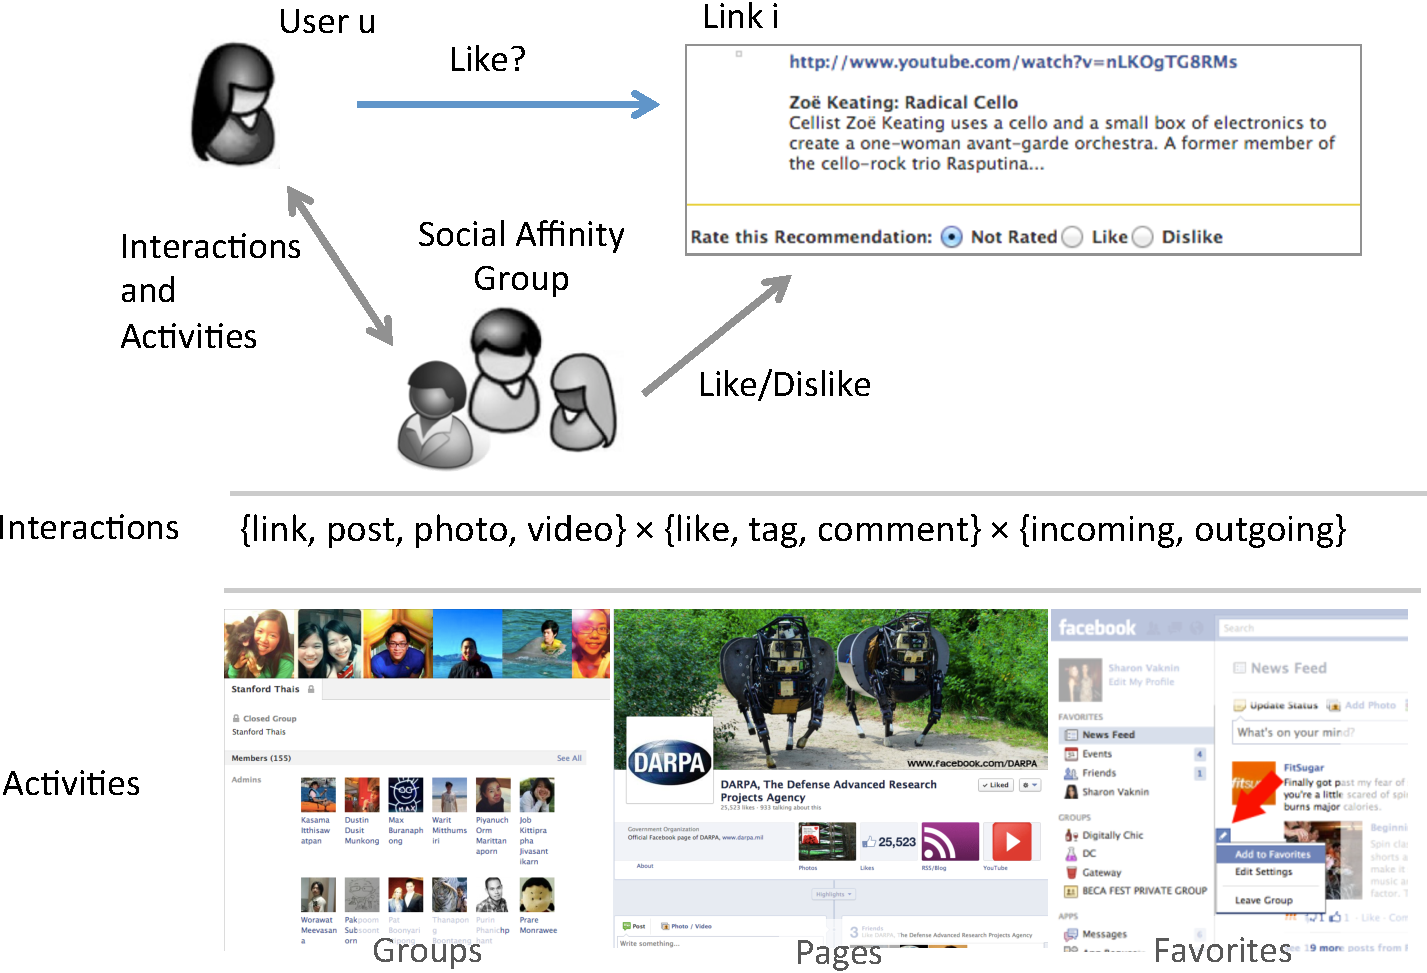
\includegraphics[width=1\linewidth]{data/overview}
\caption{Overview of social affinity for link recommendation.
A \emph{social affinity group (SAG)} consists of the set of alters 
of a user $u$ (ego) who have a
certain interaction or share an activity membership with $u$.
Alters defined by SAGs serve as proxies for an ego's interest with some
SAGs showing stronger affinity with an ego as learned by \emph{social affinity filtering (SAF)}
and analysed subsequently.}
\label{fig:overview}
\end{figure}
%%%%%%%%%%%%%%%%%%%%%%%%%%%%%%%%%%%%%%%%%%%%%%%%%%%%%%%%%%%%%%

There are a total of 22 interaction types. Namely the cross-product of modalities, actions and directions, minus {\em link-tag-\{incoming, outgoing\}} since links cannot be tagged in Facebook.

%\subsection{Activities}
%\noindent
% Can we insert more specific links to Facebook blog?  -SPS


{\bf Activities} describes the user interactions with Facebook communities like groups, pages, favourites.
\begin{itemize}
  %@SCOTT/LEXING following defination are taken from facebook blog. I am confused how to cite it %
  \item \textbf{Groups} on Facebook 
% I didnt find facebook favourites defination in facebook blog - Suvash
\footnote{From Facebook Blog: 
\surl{http://www.facebook.com/blog/blog.php?post=324706977130}, ``Groups are the place for small group communication and for people to share their common interests and express their opinion. Groups allow people to come together around a common cause, issue or activity to organize, express objectives, discuss issues, post photos and share related content''. 
\label{fn:fbblog}}
are analogous to community organizations in the real-world. It allows users to declare membership and supports people to organize activities, to post related content, and to have recurring discussions about them.  Examples of groups include {\em Stanford Thai} (Fig~\ref{fig:overview} bottom left), or {\em Harvard Debate Club}.
  \item \textbf{Pages} on Facebook
  \footnote{From Facebook Blog: 
(\surl{http://www.facebook.com/blog/blog.php?post=324706977130} ``Facebook Pages enable public figures, businesses, organizations and other entities to create an authentic and public presence on Facebook. Facebook Pages are visible to everyone on the internet by default. Facebook user can connect with these Pages by becoming a fan and then receive their updates and interact with them.'' }
  %\footnotemark[\ref{fn:fbblog}] 
  are analogous to the homepages of people, organizations and events on the world-wide-web. They are publicly visible, and users can subscribe to the updates on the page, and also engage in discussions. Example pages include {\em DARPA} (an organization, Fig~\ref{fig:overview} bottom middle), or {\em Beyonce} (a singer).

  \item \textbf{Favourites} are analogous to bookmarks (on physical books or on the web browser). It it is a user-created list containing various digital items such as Facebook apps, books, music, and many other types of items to indicate their interest. Example favourite items include {\em Big Bang Theory} (TV series), or {\em FC Barcelona} (soccer club). Fig~\ref{fig:overview} bottom right show a Facebook screenshot when a user adds a favourite.
  \footnote{According to Facebook Blog, (\surl{https://www.facebook.com/help/232262810142682} ``Facebook facilitates a wide variety of user selected favourites (Activities, Favorite Athletes, Books, Interests, Movies, Music, Sports, Favorite Teams, Television). These favourites allow a user to associate themselves with other people who share their same favourite tendencies.}
\end{itemize} 

Our evaluation includes 3000+ {\em group}, 4000+ {\em page} and 10,000+ {\em favourite} 
features as detailed in Sec~\ref{sec:datadesc}.

%% This is good text, but probably better in related work.  We have CIKM reviewers here who are
%% just skimming and trying to follow the technical setup in the initial sections... this
%% serves as a bit of a digression that detracts from some of the more important quantitative
%% points that we want to drive home with the reader as early as possible.  -SPS
\eat{
Note that the notion of affinity we adopt is based on direct user {\em actions}, rather than
static profile information, or structural information of the social graph. 
We believe this is a useful view into the social network, as it was recently pointed out
that a user's attention (i.e., interactions) are divided among a small subset of Facebook friends~\cite{backstrom2011center}, and that ratings of real-world friendship strength seems to be more predictable from the intimacy, intensity, and duration of interactions, than from social distance and structural information~\cite{gilbert2009predicting}. Our affinity definition is based on direct interactions within a users' ego network, this is complementary to 
a recent alternative~\cite{Panigrahy2012ubr} that uses number of paths between two users encodes the resilience of network structure, 
as it was recently found~\cite{Goel2012structure} that the vast majority of information diffusion
happens within one step from the source node. }
% interactions
%Our affinity
%\cite{Wilson2012BSG}


\subsection{Social Affinity Groups}
\label{ssec:sag}

\eat{
The major objective of this paper is to evaluate the effectiveness of \textit{Social Affinity Filtering (SAF)} and fine grained 
analysis of the informativeness of Interactions and Activities.We divide our recommendation algorithm into two categories based 
on Interactions and Activities of 
}

Based on the definitions of {\em interaction}  and {\em activities} above, 
%\textit{ Social Affinity Groups (SAG)} with target item, 
we define two types of {\em social affinity groups} of a user with a target item,
namely \textit{Interaction  Social Affinity Groups (ISAG)} and \textit{Activity Social Affinity Groups (ASAG)}.

\begin{itemize}
  \item \textbf{Interaction  Social Affinity Groups}. Let the set of interaction affinity classes be the cross-product of 
  Interaction modality, action and direction:
  %\begin{quote}
  \begin{align*}
  	\textit{Interaction Affinity Classes} := \, & \{\link, \post, \photo, \video\} \\
                                                & \times \{\like, \ttag, \comment\} \\
                                                & \times \{\incoming, \outgoing\}
  \end{align*}
  %\end{quote}
  %Additionally, we add friendship interaction affinity class. \\
  Then we define 
  \begin{quote}
  \textit{ISAG(u, k)} $:=$ the set of the users who have interaction $k$ with user $u$.
  \end{quote}
   For example,
   \begin{quote}
   
   \textit{ISAG(u, link-like-incoming)}  is the set of all users who have liked link posted by user $u$. \\
   \\
   \textit{ISAG(u, photo-comment-outgoing)} is the set of all users whose photos received at least one comment from $u$.
   \end{quote}
\item \textbf{Activity Social Affinity Groups}: We define activity affinity groups based on group membership, page likes and user favourites.
	\begin{quote}
	\textit{ASAG(u, k)} $:=$ the set of the users who have common preference for entity $k$ (group, page, favourite) with user $u$.   
	\end{quote}
\end{itemize}


\subsection{Social Affinity Features}
\label{ssec:SAfeature}

\begin{itemize}
  \item \textbf{Interaction Social Affinity Features} : We define Interaction affinity features for target user $u$ and item $i$ for ISAG's classes 
  $ \langle X_{1},X_{2}\ldots,X_{k}\rangle$ as
  %\begin{quote}
  \begin{equation*}
   X_{k,u,i} = \begin{Bmatrix}
   		\mathit{true} & \text{if}\ \exists v\in ISAG(u,k) \wedge likes(v,i)\\ \\
   		\mathit{false} & \text{otherwise}
   \end{Bmatrix}
  \end{equation*}
  %\end{quote}
  Additionally we add friend feature which encodes whether the target item $i$ is liked by friend or not.
  \item \textbf{Activity Social Affinity Features} : We define activity affinity features for target user $u$ and item $i$   \
  $ \langle X_{1},X_{2}\ldots,X_{k}\rangle$ as\\ \\
  \begin{equation*}
   X_{k,u,i} = \begin{Bmatrix}
   		\mathit{true} & if\ \exists\ v\in \ ASAG(u,k) \wedge likes(v,i)\\ \\
   		\mathit{false} & otherwise
   \end{Bmatrix}
  \end{equation*}
	In our analysis we use only those features (groups, pages and favourites) that are joined/liked by at least one of our app users.
\end{itemize}

\eat{
%% SCOTT already covered these elsewhere
%% Hmmm... maybe I forgot to :)  -SPS
We train naive bayes, Logistic Regression(LR) and Support Vector Machine(SVM) model with affinity features.
Logistic Regression and SVM algorithm was implemented using \textit{LIBLINER} \cite{liblinear} package. 
We define Constant predictor as baseline predictor. Constant predictor predicts the most common outcome in our datase ie disliket.
We compare the performance of Social Affinity Filtering with the state of the art social collaborative filtering technique 
Social MatchBox(SMB)\cite{SMB}.

In real world social networks activity features grows very quickly as number of user in social network increases. This motivates the fine grained
analysis of informativeness of social affinity features. Furthermore, fine grained analysis of interactions helps to understand the nature of user-user 
interactions and its predictiveness in greater detail. Hence, for the analysis of activities and interactions we rank the features using
\textit{Conditional Entropy}. 
\textit{Conditional Entropy} is defined as
\begin{quote}
\begin{math}
H(Y|X=\true) = \\-\sum_{y\in{(like,dislike)}} p(y|X$=$true)$ $log( p(y|X$=$true))
\end{math}
\end{quote}

With the data and methodology now defined including all dimensions of our analysis, we now proceed to an in-depth discussion of our findings.
}




 




